\documentclass[conference]{IEEEtran}

\usepackage[utf8]{inputenc}
\usepackage[T1]{fontenc}
\usepackage{silence}\WarningsOff[latexfont]

\usepackage{amsmath}

\RequirePackage{tikz}[2010/10/13]
\usetikzlibrary{arrows,automata,calc,intersections,patterns,decorations.pathmorphing,decorations.pathreplacing}

\usepackage{graphicx}
\usepackage{cite}
\usepackage{url}
\usepackage[caption=false,font=footnotesize]{subfig}
\usepackage[binary-units,per-mode=symbol]{siunitx}
\sisetup{list-final-separator = {, and }}
\usepackage{booktabs}
\usepackage{pifont}
\usepackage{microtype}
\usepackage{textcomp}
\usepackage[american]{babel}
\usepackage[noabbrev,capitalise]{cleveref}
\usepackage{xspace}
\usepackage{hyphenat}
\usepackage[draft,inline,nomargin,index]{fixme}
\fxsetup{theme=color}
\usepackage{grffile}
\usepackage{xfrac}
\usepackage{multirow}
\RequirePackage{xstring}
\RequirePackage{xparse}
\RequirePackage[index=true]{acro}
\NewDocumentCommand\acrodef{mO{#1}mG{}}{\DeclareAcronym{#1}{short={#2}, long={#3}, #4}}
\NewDocumentCommand\acused{m}{\acuse{#1}}
\usepackage{upquote}
\usepackage{listings}

\acrodef{DHT}{Distributed Hash Table}

\begin{document}

\title{Source Routing for \\ Downward Data Traffic}

\author{
	\IEEEauthorblockN{Andrea Zorzi [190964]}
	\texttt{andrea.zorzi-1@studenti.unitn.it}
}

\maketitle

\begin{abstract}
This report presents a simple routing protocol for tree-based topology wireless sensor networks. The protocol is intended to enable data collection from any node of the network to a sink node using multi-hop packet forwarding and at the same time, it allows to a sink node to send "command" packets downwards to any node of the network.
\end{abstract}

\acresetall

\section{Introduction}
\label{sec:introduction}

The protocol presented here has been developed with the aim of allow nodes belonging to a tree topology based wireless sensor network to exchange and forward packets coming from and towards a sink. Packets called "beacons" are periodically broadcasted by a sink node and shared between nodes in order to exchange information about the distance of each node from the sink and are used to maintain the tree topology. Beacons are are spread in a way that network traffic is minimized and nodes that change their place in space are able to reconfigure themselves and be constantly reachable by the sink.

Data collection packets are periodically send by each node to its parent until they reach the sink. 
This type of packets, meanwhile they travel through the network, are enriched with information about the the route (node addresses) they use to reach the sink. These datas are used by the sink to maintain in a routing table the knowledge about the current network topology.

"Command" packets are used by the sink node to send data to a specific node in the network. According to the current information collected in the routing table, the sink decide whether it is possible to reach a node or not and send the command packet.

The report will first describe the architecture of the network, the organization of the source code and the model of each message presented above.
Then it will explain how some major issues concerning data forwarding and packet sending are addressed by the protocol.

\section{Build and Run Network Simulation}
\label{sec:build_and_run}

The source code of the project is divided in 3 main files:

\begin{itemize}
	\item \texttt{\textbf{app.c}} Contains the code to start the main process.
	\item \texttt{\textbf{my\_collect.c}} Contains the callbacks and functions that handle the incoming and outgoing packets and deliver them to the app.
	\item \texttt{\textbf{my\_routing\_table.c}} Contains all the functions to read and update the routing table. Source code of this file is used only by the sink node.
\end{itemize}


In order to compile and build the project, the following commands should be run from the root folder of the project:
\begin{lstlisting}[language=bash] 
$ make
\end{lstlisting}

After building the project, the 2 files \texttt{test.csc} and \texttt{test\_nogui\_dc.csc} can be used to run the protocol in a simulated wireless network using \texttt{cooja}:
\begin{lstlisting}[language=bash] 
$ ./cooja test.csc
$ ./cooja_nogui test_nogui_dc.csc
\end{lstlisting}

\section{Packet Models}
\label{sec:packet_model}

Different messages are exchanged between nodes of the wireless networks.
Here are reported all the possible messages that a node could send or receive depending on its role in the network.

% Message beacon ---------------------------------------------------------------------------------
\subsection{Beacon message}

Beacon messages are used to built the tree topology of the network.

As shown in \cref{fig:msg_beacon}, every beacon contains:

% Items
\begin{itemize}

\item \textbf{seqn} The sequence number of the beacon periodically incremented by the sink.

\item \textbf{metric} And integer indicating the distance (hops) of the node which has sent the beacon from the sink.

\end{itemize}

% Figure
\begin{figure}[t]
	\centering
	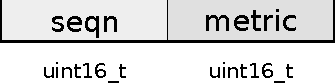
\includegraphics[width=0.5\columnwidth]{res/beacon}
	\caption{The beacon message contains two fields: \textit{seqn}  and \textit{metric}}.
	\label{fig:msg_beacon}
\end{figure}

The sink is the node that periodically broadcast beacon packets.
When a node  of the network receive a beacon, it analyzes the beacon's payload, its RSSI and decide if the packet is fresh enough to be take into consideration and to be retransmitted to other nodes. More details are described in the next section.


% Message data collection and command -------------------------------------------------------------

\subsection{Common messages}

The other messages that are exchanged between nodes, apart from beacons, have all the same structure and depending on the content of the header they have different meanings. 
The header is composed by two parts: the first has a fixed size while the second is an array of node addresses that, depending on its content, it have different lengths.

All the fields of packet are shown in \cref{fig:msg_packet} and described here:

\begin{itemize}

\item \textbf{source} Contains the address of the node which sent the packet.

\item \textbf{hops} Contains a counter incremented every time the packet is forwarded to another node.

\item \textbf{is\_command} A boolean flag that allows nodes to distinguish \texttt{command} packets typically sent by the sink from others messages.

\item \textbf{path\_length} Indicates the length of the array contained in bytes that immediately follow this field.

\item \textbf{path} All the bytes contained between the \texttt{path\_length} field and \texttt{data} are interpreded as an array of node's addresses. Depending on the type of packet, the array can be used by the sink to populate and update its routing table or it can contain the route that the packet should follow to reach its destination.

\item \textbf{data} The \texttt{data} part of the packet contains the payload read by the destination node.

\end{itemize}

% Figure
\begin{figure}[t]
	\centering
	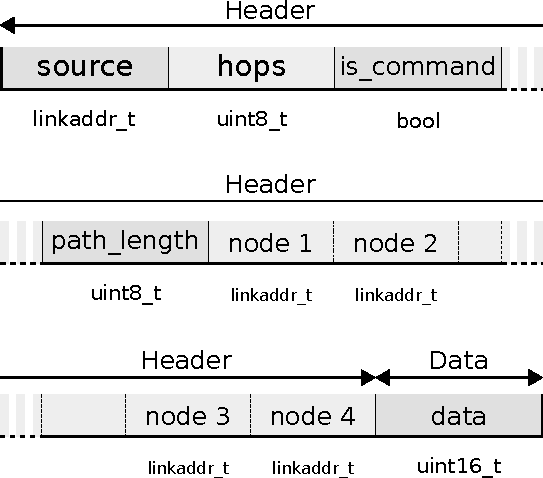
\includegraphics[width=0.8\columnwidth]{res/msg}
	\caption{Representation of a common packet exchanged by nodes. It is divided in header part and data part.}
	\label{fig:msg_packet}
\end{figure}

Here are described the different types of messages:

\begin{itemize}

\item \textbf{Data Collection Packets} This type of message is sent by any node that at certain time needs to report to the sink some data. The \textit{sender} node attaches to the message the data that has to send. In the header it specifies itself as the source, it initializes the hop field and insert its address in the array of node's addresses. 

Whenever one of the other nodes receives a message of this type, it tries to forward the packet to its parent until it reaches the sink. Before forwarding the packet, each node insert its address in the \texttt{path} array.

\item \textbf{Topology Report Packets} Topology Report packets are sent by every node to inform the sink about the current network topology. This kind of packets are similar to the Data Collection packets. They differs from the previous tipology only beacuse the \texttt{data} part of the packet is empty.

\item \textbf{Command Packets} These packets are used by the sink to send to a specific node in the network some data. The header's \texttt{path} field is filled with the route that the packet should follow to reach its destination. The \texttt{is\_command} flag is set to \textit{true} to inform the nodes to handle this packet differently from the other ones.

\end{itemize}




\section{Architecture}
\label{sec:architecture}

Here are discussed in details some of the aspects that caracterize the protocol and how nodes handle incoming packets.

\subsection{Beacon handling}

When a beacon packet is received by any node, it is analyzed and dropped or forwarded depending on some factors.

Beacons that have an RSSI value lower than a certain threshold (-95 dB) are discarded.

Depending on the sequence number (\texttt{seqn} header field) contained in the packet, the beacon is handled in different ways:

\begin{itemize}

\item If the value is lower than the last one registered by the node, beacon is considered old and it is discarded.

\item If the value is greater than the last one registered by the node, it means that the beacon contains "more updated" information about the network topology. In this case, the parent's node is updated and become the node from which the beacon comes from. This decision allow the node to be always connected to a parent in contact with the sink even if its position in the network changes in time. In this case the \texttt{metric} field contained in the beacon is not taken in consideration.

\item If the value is equal than the last one registered by the node, \texttt{metric} value is used to decide whether update or not the parent. The parent of the node is replaced with the beacon's sender in two cases: the beacon must have a greater metric than the current parent's node or, if the two metric values are equal, the beacon RSSI must be greater than the one of the current parent.

\end{itemize}

In any case, every time the parent is updated with a new one, the node broadcast the beacon over the network. A random delay before send the packet is used to avoid collisions with beacons broadcast by other nodes.


\subsection{Routing table and topology discovery}

The sink node maintains a routing table used to send unicast packets to nodes. The routing table is updated thanks to dedicated topology report packets or using piggybacking. In the latter case, sink uses the data contained in data collection packets to discover the parent-child relationships between nodes. In fact, data collection packets have a \texttt{path} field that contains an array of node's addresses that is populated by every node that forwarded the packet with its address. The sink can read this field and obtain the a chain of nodes from which the packet is pass through from child to parent before reaching its destination.

Notice that the \texttt{path} field contained in every packet is also used by halfway nodes to detect loops. If the \texttt{path} array already contains the address of the node that is handling the packet, it means that it is already passed through the current node and so it is dropped.


\subsection{Dedicated Topology Report}

Every node sends dedicated topology reports to the sink when it update its parent to inform the sink about changes in network topology. Reports are sent after a random delay which is lower the most the node is far from the sink (in term of hop counts).
A node may receive topology reports from children asking it to forward reports to the sink. In this case, if the node has a pending report to send (due to the delay), it drops its own report and attach its information to the child's report and forwards it. This allows to avoid duplicated information and reduce the number of topology reports exchanged in the network in a certain period of time.


\subsection{Source Routed Packets (Commands)}

Sink can send unicast packets to any node in the network. Information to calculate the route that the packet should follow to reach the node are stored in the sink's routing table. They are used to iteratively fill the route array adding the address of the next node that will forward the packet until the recipient node is reached. At every iteraction step, the sink verify that in the partially built route array no addresses are present more than one time. Otherwise a loop is detected and the dispatch of the packet is interrupted. The route array is then stored in the \texttt{path} field of the packet. 

Since nodes of the network do not know the address of the sink, they can not infer from the \texttt{source} field that the packet comes from the sink and should be forwarded to the next node in the route array. In order to find a solution to this problem, the \texttt{is\_command} field is used and set to true by the sink. This allows to distinguish packets that should reach the sink from packets that should reach other nodes of the network tree.





\section{Conclusions}
\label{sec:conclusions}

The project aims to build a simple protocol that supports data collection and allows the sink to send packets to specific nodes of the wireless network.
Despite its simplicity, the protocol can be easily extended to cover other scenarios. For example, thanks to the \texttt{is\_command} flag contained in header of every packet, any node (and not only the sink) could have the chance to send unicast packets.
\section{Some Results}
\label{sec:some_results}

The protocol has been tested using \texttt{cooja}. Here are reported some results:

\subsection{Using RDC: NullRDC}

\begin{lstlisting} 
--- Data Collection Overall Statistics ---
Total Number of Packets Sent: 531
Total Number of Packets Received: 527
Overall PDR = 99.25%
Overall PLR = 0.75%


--- Source Routing Overall Statistics ---
Total Number of Packets Sent: 172
Total Number of Packets Received: 171
Overall PDR = 99.42%
Overall PLR = 0.58%
\end{lstlisting}


\subsection{Using RDC: ContikiMAC}

\begin{lstlisting} 
--- Data Collection Overall Statistics ---
Total Number of Packets Sent: 531
Total Number of Packets Received: 480
Overall PDR = 90.40%
Overall PLR = 9.60%

--- Source Routing Overall Statistics ---
Total Number of Packets Sent: 173
Total Number of Packets Received: 169
Overall PDR = 97.69%
Overall PLR = 2.31%
\end{lstlisting}


\end{document}

